\section{Desarrollo}
\subsection{Circuito I: VFA-VFA}
\hspace{1mm} El amplificador operacional que se implementa para el circuito propuesto es el LM328 para el circuito propuesto.  integrados que se utilizan para el amplificador VFA es el LM324 cuyas especificaciones se detallan a continuación.

\begin{itemize}
    \item \(A_{d0}=100~dB\)
    \item \(F_T=1~MHz\)
    \item \(F_1=10~Hz\)
    \item \(F_2=5.06~MHz\)
\end{itemize}

\bigskip
\hspace{1mm} Seguidamente, se calculará la ganancia del circuito considerando el segundo AO como ideal. Para ello, se deberán calcular las ganancias de lazo abierto \(Ad(s)\), ganancia de lazo \(T(s)\) y ganancia de lazo cerrado \(Avf(s)\). Con todos estos datos se procederá a compensar el amplificador compuesto para lograr una máxima planicidad de módulo.

\begin{figure}[H]
    \centering
    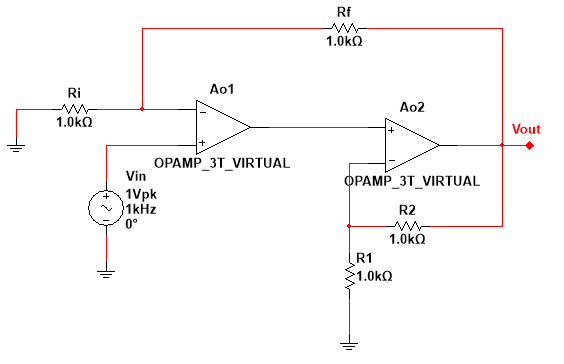
\includegraphics[width=0.7\linewidth]{VFA-VFA-Circuito.png}
    \caption{Amplificador VFA-VFA}
    \label{fig:enter-label}
\end{figure}

\hspace{1mm} Se obtiene la ganancia de lazo abierto. Esta misma es la relación entre la tensión de salida y la tensión de entrada.

\begin{equation}
    Av(s) = \frac{V_{out}}{V_{in}}
\end{equation}

\bigskip
\hspace{1mm} Se obtienen las expresiones de las tensiones \(V_{o1}\) y \(V_{o2}\).

\begin{equation}
    V_{o1} = Ad(s)\cdot V_{in} 
\end{equation}

\begin{equation}
     V_{o2} =V_{out}= V_{o1}\cdot \Bigl(1+\frac{R_2}{R_1}\Bigl)
\end{equation}

\begin{equation}
    V_{o2} =V_{out}= Ad(s) \cdot V_{in} \cdot \Bigl(1+\frac{R_2}{R_1}\Bigl)
\end{equation}

\hspace{1mm} La relación entre la salida y la entrada da como resultado la ganancia de lazo abierto.

\begin{equation}
    \boxed{
    Av(s) = Ad(s)\cdot \Bigl(1+\frac{R_2}{R_1}\Bigl)
    }
\end{equation}

\bigskip
\hspace{1mm} Luego, se calcula la ganancia de lazo T.

\bigskip
    \[T(s) = \frac{V_{out}}{V_{out'}}|_{V_{in}=0}\]

\hspace{1mm} Entonces.
\[V_{o1}= Ad(v^+-v^-)\]
\[V_{o1}= Ad.\Bigl(0V-V_{o}'\frac{R_i}{R_i+R_f}\Bigl)=-Ad.V_{o}'\Bigl(\frac{R_i}{R_f}+1\Bigl)\]
\begin{equation}\label{eq:primera_etapa} 
\boxed{V_{o1} = -Ad.V_{o}'\Bigl(\frac{R_i}{R_f}+1\Bigl)}
\end{equation}

\bigskip
\hspace{1mm} Luego, \(V_{out}\)  ha sido calculado para la ganancia de lazo abierto.

\begin{equation}
    V_{out}= V_{o1}\cdot \Bigl(1+\frac{R_2}{R_1}\Bigl)
\end{equation}

\hspace{1mm} Por lo tanto, 

\begin{equation}
    \boxed{
      T(s) = -Ad(s)\cdot \Bigl(\frac{R_2}{R_1}+1\Bigl)\cdot \Bigl(\frac{R_i}{R_f}+1\Bigl)
    }
\end{equation}
  
\bigskip
\hspace{1mm} Se tiene que la ganancia de lazo cerrado es:

\begin{equation}
    Avf(s) = \frac{Av(s)}{1-T}
\end{equation}

\begin{equation}
      Avf(s) = \frac{Ad(s)\cdot \Bigl(\frac{R_2}{R_1}+1\Bigl)}{1+Ad(s)\cdot \Bigl(1+\frac{R_2}{R_1}\Bigl)\cdot \Bigl(\frac{R_i}{R_f}+1\Bigl)}
\end{equation}

\bigskip
\hspace{1mm} Considerando la ganancia \(Ad(s)\) tiende a infinito, se simplifican los cálculos referidos a la ganancia de lazo cerrado.

\bigskip
\begin{equation}
      Avf(s) = \lim_{Ad(s)\to\infty} \frac{Ad(s)\cdot (\frac{R_2}{R_1}+1)}{1+Ad(s)\cdot (1+\frac{R_2}{R_1})\cdot \Bigl(\frac{R_i}{R_f}+1\Bigl)}
\end{equation}
\begin{equation}
    \boxed{
        Avf(s)=\Bigl(\frac{R_f}{R_i}+1\Bigl) 
    }
\end{equation}

\bigskip
\hspace{1mm} El requerimiento con respecto a la ganancia es que debe ser \(Avf(s)=20~dB\). Con este dato, se obtiene la relación entre lasf resistencias \(R_i\) y \(R_f\).
\begin{equation}
    Avf(s)=20~dB
\end{equation}
\begin{equation}
    20~dB=20\cdot\log{(Avf)}
\end{equation}
\begin{equation}
    \log{(Avf)}=\frac{20~dB}{20}
\end{equation}
\begin{equation}
    \log{(Avf)}=1
\end{equation}
\begin{equation}
    Avf=10
\end{equation}
\begin{equation}
    \Bigl(\frac{R_f}{R_i}+1\Bigl)=10
\end{equation}
\bigskip
\hspace{1mm} Despejando la relación de resistencias.
\bigskip
\begin{equation}
    \frac{R_f}{R_i} = 9 \hspace{7mm} R_f=R_i \cdot 9
\end{equation}
\begin{equation}
    R_f=R_i \cdot 9
\end{equation}

\bigskip
\hspace{1mm} Se colocan valores arbitrarios de resistencias que cumplan con la relación anteriormente hallada.

\begin{equation}
    \boxed{
        R_i=10~k\Omega \hspace{3mm} , R_f=90~k\Omega
    }
\end{equation}

\bigskip

\hspace{1mm} Se realiza la simulación en Python de la función transferencia del amplificador operacional.

\begin{lstlisting}[language=Python]
import numpy as np
import plotly.graph_objects as go
from scipy import signal

# Variables
Ado = 100  # dB
f1 = 10  # Hz
f2 = 5.06e6  # Hz

w1 = 2 * np.pi * f1
w2 = 2 * np.pi * f2

num = 10 ** (Ado / 20)
den = [1 / (w1*w2), 1/w1 + 1/w2, 1]

# Crear sistema
Av = signal.TransferFunction(num, den)

# Bode
w = np.logspace(-1, 10, 1000)
w_v, mag_v, phase_v = signal.bode(Av, w)
f_v = w_v / (2 * np.pi)

# Crear grafico
fig = go.Figure()
# Magnitud
fig.add_trace(go.Scatter(
    x=f_v,
    y=mag_v,
    mode='lines',
    name='Magnitud [dB]',
    line=dict(color='blue')
))
# Fase
fig.add_trace(go.Scatter(
    x=f_v,
    y=phase_v,
    mode='lines',
    name='Fase [deg]',
    yaxis='y2',
    line=dict(color='red')
))
# Configurar los ejes
fig.update_layout(
    title="Bode Plot",
    xaxis=dict(
        title="Frecuencia [Hz]",
        type="log",
    ),
    yaxis=dict(
        title="Magnitud [dB]",
        side="left"
    ),
    yaxis2=dict(
        title="Fase [deg]",
        overlaying="y",
        side="right"
    ),
    legend=dict(x=0.75, y=0.95),
    template="plotly_white"
)
fig.show()
\end{lstlisting}
\bigskip

\hspace{1mm}  De éste script se obtiene el diagrama de Bode de la función transferencia de lazo abierto del amplificador operacional (LM324). El amplificador operacional anteriormente nombrado tiene un polo en \(10~Hz\) y otro en \(5.06~MHz\).

\begin{figure}[h!]
  \centering
    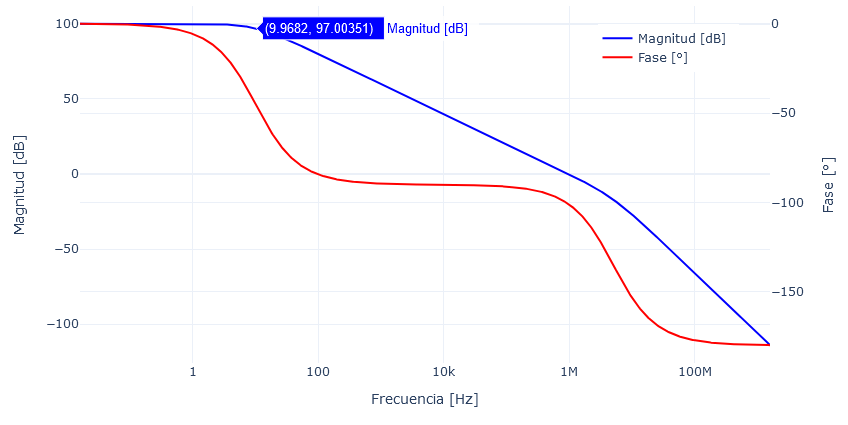
\includegraphics[scale=0.7]{TP3_bode_lm324.png}
    \caption{Diagrama de Bode del amplificador lazo abierto}
\end{figure}

\bigskip
\hspace{1mm} Se tiene que uno de los requerimientos es que se debe tener máxima planicidad de módulo \(M\varphi =65°\).  A lazo cerrado se encuentra un polo en \(f_g\) el cual esta relacionado con la ganancia del amplificador \(A_{o2}\).
\bigskip

\hspace{1mm} Se considera que el amplificador \(A_{o2}\) es ideal. determinando a continuación la fórmula del margen de fase de la cual se despejó el polo \( 
f_g \)
 
\begin{equation}
    M \varphi = 360^o - 180^o - arctg \left( \frac{f_g}{f_1} \right) - arctg \left( \frac{f_g}{f_2} \right) = 65^o
\end{equation}
\begin{equation}
    M \varphi = 180^o - arctg \left( \frac{f_g}{f_1} \right) - arctg \left( \frac{f_g}{f_2} \right) = 65^o
\end{equation}
\begin{equation}
    115^o = arctg \left( \frac{f_g}{f_1} \right) + arctg \left( \frac{f_g}{f_2} \right)
\end{equation}
\begin{equation}
    \boxed{
    f_g = 2,36~MHz
    }
\end{equation}
\bigskip
\hspace{1mm} Se determinó la ganancia a lazo cerrado del amplificador \(A_{O2}\) ideal de la siguiente manera. Considerar que la ganacia de lazo cerrado ideal fue dada en la consigna y es la siguiente \((Avfi=20~dB)\).


\begin{equation}
    Avf_{2i}=\frac{Avfi \cdot \omega_{gi}}{Ad_0 \cdot \omega_1} = 27~dB
\end{equation}

\bigskip
\hspace{1mm} Este valor de ganancia se utilizó para obtener la ganancia del amplificador compuesto.

\begin{equation}
    Av_{comp}=Ad0\cdot Avf_{2i}=100~dB \cdot 27~dB
\end{equation}

\begin{equation}
    \boxed{
    Av_{comp} = 127~dB
    }
\end{equation}

\bigskip

\hspace{1mm} Se diseña la función de transferencia de lazo cerrado del amplificador compuesto \(A_{vf_{comp}}\). Se determina la ganancia de ruido global \(K_{global}\).

\[20~dB= 20 \log(A_{vf_{comp}})\]
\[\log(A_{vf_{comp}})=\frac{20~dB}{20}\]
\[A_{vf_{comp}}=10^{1}\]
\[A_{vf_{comp}}=10\]
\begin{equation}
    K_{global} = \frac{1}{A_{vf_{comp}}} = \frac{1}{10}
\end{equation}
\begin{equation}
    \boxed{
    K_{global} = 0.1
    }
\end{equation}

\bigskip
\hspace{1mm} Se resolvió así la función de transferencia mencionada.

\begin{equation}
    FtAvf (comp) = \frac{Ad_0 \cdot Avf_{2i} \cdot \omega_1 \cdot \omega_2}{s^2 + s \cdot (\omega_1 + \omega_2) + (\omega_1 \cdot \omega_2 + K (global) \cdot Ad_0 \cdot Avf_{2i} \cdot \omega_1 \cdot \omega_2)}
\end{equation}

\begin{equation}
    A_{vf_{comp}}(s) = \frac{4,714 \cdot 10^{15}}{s^2 + 3,179 \cdot 10^7 \cdot s + 4,713 \cdot 10^{14}}
\end{equation}

\bigskip
\hspace{1mm} Dicha función transferencia se compara con la expresión de un sistema de segundo orden:
\begin{equation}
    A_{v}(s) = \frac{\omega _p^2}{s^2 + s \frac{\omega _p}{Q_p } + \omega_p^2}
\end{equation}  
\bigskip
\hspace{1mm} Se igualan las ecuaciones y se determinan los siguientes parámetros:
\begin{equation}
    \omega _p ^2 = 4,713 \times 10^{14} \Longrightarrow \omega_p =\sqrt{4,713 \times 10^{14}} 
\end{equation}
\begin{equation}
    \boxed{
        \omega_p = 21,7 \cdot 10^6 \space \frac{rad}{seg} 
    }
\end{equation}
\bigskip
\hspace{1mm} Entonces, la frecuencia del polo compensado es:

\begin{equation}
    f_p = \frac{\omega_p}{2\pi}=\frac{21,7 \cdot 10^6 \frac{rad}{seg}}{2\pi}
\end{equation}

\begin{equation}
    f_p = 3,45\cdot 10^6 \space Hz= 3,45\space MHz
\end{equation}
\begin{equation}
    \boxed{
    f_p = 3,45\space MHz
    }
\end{equation}

\bigskip
\hspace{1mm} Se comprueba que \( Q_p \).

\begin{equation}
    3,179 \cdot 10^7 \frac{rad}{seg} = \frac{\omega_p}{Q_p} 
\end{equation}
\begin{equation}
    Q_p = \frac{\omega_p}{3,179 \cdot 10^7} = \frac{21,7 \cdot 10^6 \frac{rad}{seg}}{3,179 \cdot 10^7} = 0,696 \approx 0,7
\end{equation}

\begin{equation}
    \boxed{
    Q_p = 0,7
    }
\end{equation}

\hspace{1mm} Se tiene que la caída de los \(-3~dB\) se tiene a una frecuencia de \(f_p=300KHz\) aproximadamente.

\hspace{1mm} Como la ganancia de lazo cerrado es igual a \(Avf_2=27~dB\) y, por lo tanto, la ganancia del amplificador compuesto a lazo abierto resulta ser \(127~dB\). Con estos valores, se puede calcular el valor del polo \(f_g\).

\begin{equation}
    \frac{127~dB-20~dB}{log(10)-log(f_g)}=-20~dB/dec
\end{equation}

\bigskip
\hspace{1mm} Se despeja \(f_g\), y se obtiene:

\begin{equation}
\boxed{
    f_g=2.2~MHz
}
\end{equation}

\hspace{1mm} Considerando que \(A_{vf2}=27~dB\). Entonces se tiene que la ganancia en veces será.

\[27~dB= 20 \log(A_{vf2})\]
\[A_{vf2}=10^{1.35}\]
\[A_{vf2}=22,38\]
\[\Bigl( {\frac{R_2}{R_1}+1} \Bigl)=22,38\]
\[\frac{R_2}{R_1}=21,38\]
\[R_2=21,38 \cdot R_1\]
\[R_2 = 21,38 \cdot 1k\Omega\]
\[R_2 = 21,38k\Omega\]

En la siguiente figura se muestra la frecuencia de corte \(f_p=466.27KHz\) con caída de \(-3~dB\). 


\begin{figure}[H]
    \centering
    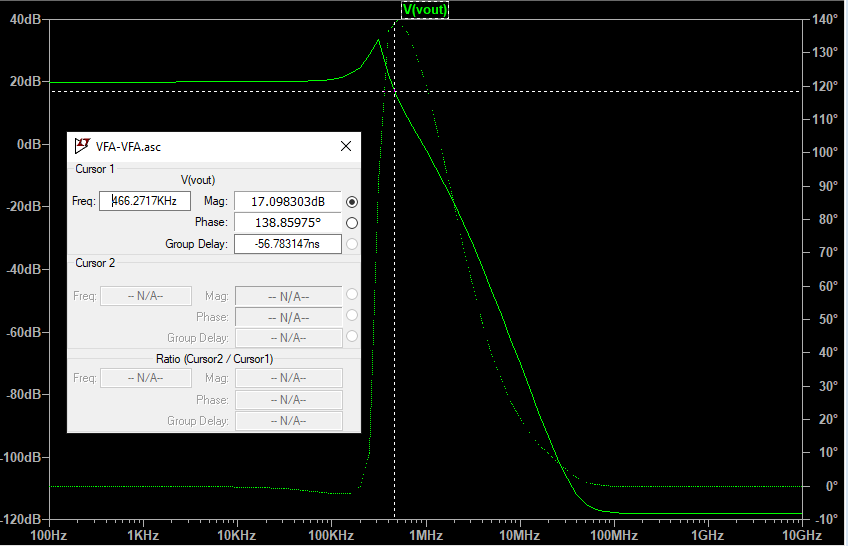
\includegraphics[width=0.7\linewidth]{VFA-VFA-Bode.png}
    \caption{Diagrama de Fase y Bode del Amplificador Compuesto}
    \label{fig:enter-label}
\end{figure}

Se concluye que no puede obtenerse la condición de compensación requerida con la condición de máxima planicidad de módulo debido a que los polos de los amplificadores operacionales se encuentran en los mismos valores \(f_1, f_2\) por lo que se necesita un amplificador operacional para la etapa 2, tal que tenga polos de mayor valor que los del LM324 \(f_1= 10Hz , f_2= 5,06MHz\).


\newpage
\subsection{Circuito II: VFA-CFA}
\hspace{1mm} El amplificador operacional que se implementa para el circuito propuesto es el LM6181 (CFA) cuyas especificaciones se detallan a continuación.

\begin{itemize}
    \item \(R_T=2.37~M\Omega\)
    \item \(C_T=4.8~pF\)
    \item \(F_1=14~KHz\)
    \item \(F_2=82.3~MHz\)
\end{itemize}

\bigskip
\hspace{1mm} Se considera que el amplificador operacional LM324 (VFA) se comporta de la misma manera que en el caso anterior  y que el polo de mayor frecuencia del CFA tiene un efecto despreciable sobre la respuesta del amplificador a lazo cerrado.

\bigskip
\hspace{1mm} La ecuación de margen de fase para máxima planicidad de módulo se desarrolla de la siguiente manera:

\begin{equation}
    M \varphi = 360^o - 180^o - arctg \left(\frac{f_g}{f_{1VFA}}\right) - arctg \left(\frac{f_g}{f_{2VFA}}\right) - arctg \left(\frac{f_g}{f_{CFA}}\right) = 65,5^o
\end{equation}

\bigskip
\hspace{1mm} Reemplazando por los valores dados.

\begin{equation}
    65,5^o = 180^o - arctg \left(\frac{2~MHz}{10~Hz}\right) - arctg \left(\frac{2~MHz}{5,06~MHz}\right) - arctg \left(\frac{2~MHz}{f_{CFA}}\right)
\end{equation}
\begin{equation}
    65,5^o = 180^o - 90^o - 21,57^o - arctg \left(\frac{2~MHz}{f_{CFA}}\right)
\end{equation}

\begin{equation}
    arctg\left(\frac{2~MHz}{f_{CFA}}\right) = 180^o - 90^o - 21,57^o - 65,5^o
\end{equation}
\begin{equation}
    arctg\left(\frac{2~MHz}{f_{CFA}}\right) = 2,93^o
\end{equation}
\begin{equation}
    tg (2,93^o) = \frac{2~MHz}{f_{CFA}}
\end{equation}
\bigskip
\hspace{1mm}Se tiene que la frecuencia del polo generado por el amplificador CFA es la siguiente:
\begin{equation}
    f_{CFA} = \frac{2~MHz}{tg (2,93^o)} = 39~MHz
\end{equation}
\bigskip
\hspace{1mm} Para obtener una máxima planicidad de módulo, la frecuencia del polo de lazo cerrado del CFA debe ser.
\begin{equation}
    \boxed{
        f_{CFA} = 39~MHz
    }
\end{equation}
\bigskip
\hspace{1mm} Como se conoce la frecuencia del amplificador CFA \((f_{CFA})\) . Se calcula la resistencia \( R_2 \) partiendo de la siguiente fórmula.
\begin{equation}
    \omega _{CFA} = \frac{1}{C_T \cdot R_2}
\end{equation}
\begin{equation}
    R_2 = \frac{1}{C_T \cdot 2\pi f_{CFA}} = \frac{1}{4,8~pF \cdot 2\pi \cdot 39~MHz}
\end{equation}
\begin{equation}
    \boxed{
        R_2 = 850~\Omega
    }
\end{equation}
\bigskip
\hspace{1mm} Se calcula la resistencia \( R_1 \) . En primera instancia, se calcula la ganancia Avf2.
\begin{equation}
    Avf \cdot f_g = Ado \cdot f_1 \cdot Avf_2
\end{equation}
\bigskip
\hspace{1mm} Se calcula la ganancia ideal de lazo cerrado del amplificador CFA \(( Avf_2)\). Se despeja la misma de la fórmula anterior.

\begin{equation}
    Avf_2 = \frac{Avf \cdot f_g}{Ado \cdot f_1} = \frac{10 \cdot 2~MHz}{100000 \cdot 10~Hz}
\end{equation}
\begin{equation}
    \boxed{
    Avf_2 = 20
    }
\end{equation}
\bigskip
\hspace{1mm} Finalmente, se calculará \( R_1 \) partiendo de la siguiente ecuación.

\begin{equation}
    Avf_2 = \Bigl(1 + \frac{R_2}{R_1}\Bigl) = 20
\end{equation}
\begin{equation}
    \frac{R_2}{R_1} = 20-1
\end{equation}
\begin{equation}
    R_1 =\frac{R_2}{19}
\end{equation}
\begin{equation}
    R_1 =\frac{850\Omega}{19}
\end{equation}
\begin{equation}
    R_1 =44,73\Omega \approx 45\Omega
\end{equation}
\begin{equation}
    \boxed{
    R_1 =45\Omega
    }
\end{equation}
\bigskip
\hspace{1mm} Como se vio en el marco teórico, al trabajar en máxima planicidad de módulo la frecuencia del polo de la función de transferencia a lazo cerrado se obtiene a partir de la siguiente expresión.

\begin{equation}
    \omega _G = 0,644 \cdot \omega _p 
\end{equation}

\bigskip
\hspace{1mm} Se especifica para el diseño que el ancho de banda potencial que se requiere es de \( f_G = 2~MHz \). Por lo tanto reemplazando y despejando de la ecuación anterior \( f_p \).

\begin{equation}
    2\pi f_G = 0,644 \cdot 2\pi f_p \Longrightarrow f_p = \frac{f_G}{0,644} = \frac{2~MHz}{0,644}
\end{equation}

\begin{equation}
    \boxed{
    f_p = 3,1~MHz
    }
\end{equation}

\bigskip
\hspace{1mm} El ancho de banda a -3dB es igual a la frecuencia del polo a lazo cerrado, que en este caso es de 3.1 MHz, ya que esta es una condición que busca maximizar la planicidad del módulo.

\subsubsection{Simulaciones}

\hspace{1mm} Se realizó la simulación del circuito propuesto en el software LTSpice. Se tiene para este caso que se implementan los amplificadores operacionales LM324 (VFA) y LM6181 (CFA).

\begin{figure}[H]
    \centering
    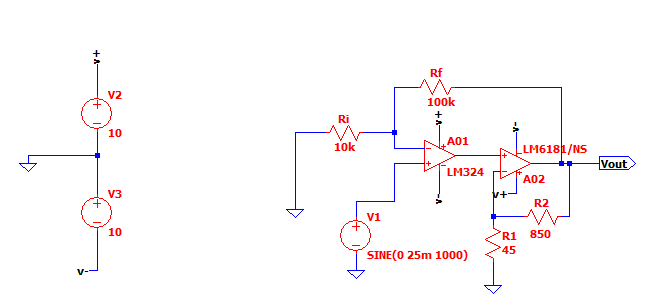
\includegraphics[width=0.7\linewidth]{VFA-CFA-Simulacion.png}
    \caption{Amplificador Compuesto}
    \label{fig:enter-label}
\end{figure}

\hspace{1mm} Se inyectó una señal sinusoidal con un valor de tensión pico de \(25~mV\) con una frecuencia de \( 1~kHz \).  Se obtienen las siguientes mediciones.


\hspace{1mm} En donde se puede comprobar que para un valor de entrada de \( 25~mV \) se obtiene a la salida \( 248~mV \) con lo cual la ganancia obtenida es:

\begin{figure}[H]
    \centering
    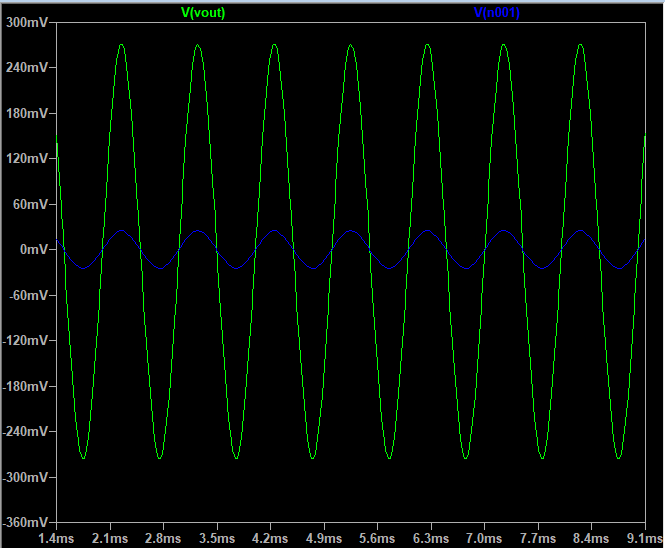
\includegraphics[width=0.7
    \linewidth]{VFA-CFA-Ganancia.png}
    \caption{Ganancia del Circuito }
    \label{fig:enter-label}
\end{figure}

\begin{equation}
    G = \frac{248~mV}{25~mV}
\end{equation}
\begin{equation}
    \boxed{
    G = 10
    }
\end{equation}

\hspace{1mm} Se realiza el diagrama de bode del circuito propuesto. 

\begin{figure}[H]
    \centering
    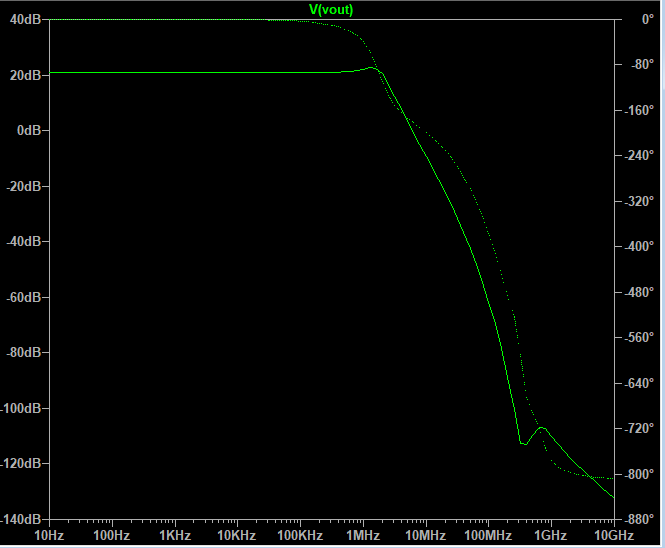
\includegraphics[width=0.7\linewidth]{VFA-CFA-Bode.png}
    \caption{Diagrama de Fase y Bode}
    \label{fig:enter-label}
\end{figure}

\hspace{1mm} Se observa una ganancia de \(20~dB\) y una caída de \(-3~dB\) a la frecuencia de \(2.7~MHz\) con fase \(-137°\).

\begin{figure}[H]
    \centering
    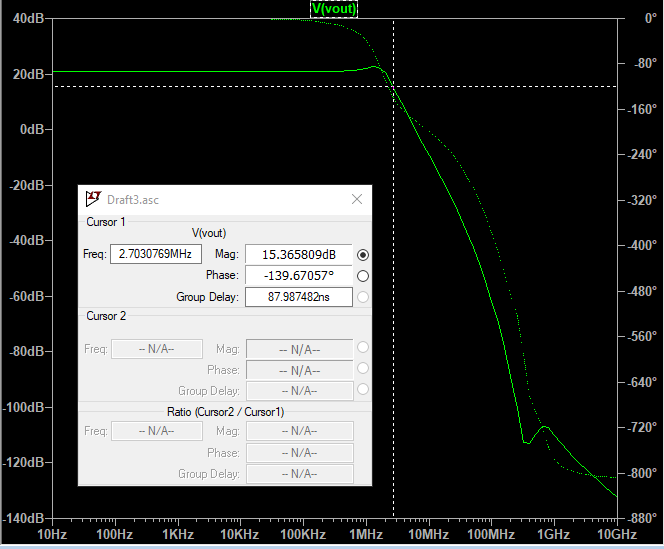
\includegraphics[width=0.7\linewidth]{VFA-CFA-Bode2.png}
    \caption{Frecuencia a una caída de -3dB}
    \label{fig:enter-label}
\end{figure}









\newpage
\subsection{Circuito III: VFA-CFA}

\hspace{1mm} Se diseña una red de compensación cero-polo, con el propósito de cancelar el polo ubicado en \(5.06~MHz\) del amplificador VFA y lograr tener en la frecuencia \(f_g= 2Mhz\). La configuración de esta red se presenta en la siguiente figura:

\begin{figure}[!h]
    \centering
    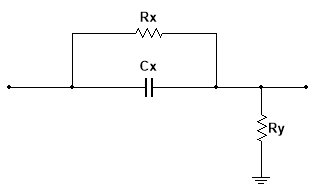
\includegraphics[width=0.5\linewidth]{img/Red de compensacion RC.png}
    \caption{Red de Compensación RC.}
\end{figure}

\hspace{1mm} Se aplica esta red de compensación (cero - polo) para compensar el efecto del polo existente en la frecuencia de \(5.06~MHz\).

\bigskip
\hspace{1mm} La función de transferencia de la red que se aplica es la siguiente:

\begin{equation}
    A_c(s) = \frac{R_y}{R_x + R_y} \cdot \frac{1 + sC_x R_x}{1 + sC_x (R_x // R_y)}
\end{equation}

\hspace{1mm} Donde se han definido las siguientes notaciones:

\begin{itemize}
    \item \(k_{comp}=\frac{R_y}{R_x + R_y}\)
    \item \( \omega_{pcomp} =  \frac{1 }{1 + sC_x (R_x // R_y)}\)
    \item \(\omega_{zcomp} = \frac{1 }{ C_xR_x}\)
\end{itemize}

\hspace{1mm} Como el cero del compensador debe cancelar el polo de frecuencia más alta del VFA, entonces:
\begin{equation}
    \omega_{zcomp} = \omega_2 = 2\pi \cdot 5.06~Mrps
\end{equation}
\hspace{1mm} El polo de compensación se encuentra una octava por encima de este cero para mantener la relación de ganancia especificada en el marco teórico. Entonces:

\begin{equation}
    \omega _{pcomp} = 2\omega _{zcomp} = 2\pi \cdot 10.12~Mrps
\end{equation}

\hspace{1mm} A partir de estos valores se pudo calcular la ganancia del compensador \(k_{comp}\)

\begin{equation}
    k_{comp} = \frac{\omega_{zcomp}}{\omega _{pcomp}} = \frac{2\pi \cdot 5.06~Mrps}{2\pi \cdot 10.12~Mrps}
    \end{equation}
\begin{equation}
    \boxed{
    k_{comp} = 0.5
    }
\end{equation}
\hspace{1mm} Por lo tanto, \(k_{comp}\) es.

\begin{equation}
    k_{comp} = \frac{R_y}{R_x + R_y} = 0.5
\end{equation}

\hspace{1mm} Se obetiene la relación entre las resistencias.

\begin{equation}
    \frac{R_y}{R_x + R_y} = \frac{1}{2} \Longrightarrow 2R_y = R_x + R_y \Longrightarrow 2 = \frac{R_x}{R_y} + 1
\end{equation}

\begin{equation}
    \boxed{
    1 = \frac{R_x}{R_y}
    }
\end{equation}

\hspace{1mm} Entonces, se consideran los siguientes valores:

\begin{equation}
    \boxed{
    R_x = R_y = 1~k\Omega
    }
\end{equation}

\hspace{1mm} Con dichos valores se puede calcular el capacitor \(C_x\) despejando la fórmula de \(\omega_{zcomp}\).

\begin{equation}
    \omega_{zcomp} = \frac{1}{C_x R_x} = 2\pi \cdot 5.06~Mrps
\end{equation}

\begin{equation}
    C_x = \frac{1}{2\pi \cdot 5.06~Mrps \cdot 1~k\Omega}
\end{equation}

\begin{equation}
    \boxed{
    C_x = 31~pF
    }
\end{equation}

\hspace{1mm} Se agrega el compensador y se obtiene la siguiente función de transferencia del lazo de realimentación: ---------

\begin{equation}
    T(s) = -A_d(s) \cdot A_c(s) \cdot A_{vf2} (s) = - \frac{kA_d(0)}{\left(1+\frac{s}{\omega_1}\right)\left(1+\frac{s}{\omega_2}\right)} \cdot k_{comp} \frac{\left(1 + \frac{s}{\omega_{zcomp}}\right)}{\left(1+\frac{s}{\omega_{pcomp}}\right)} \cdot A_{vf2}(s)
\end{equation}

\hspace{1mm} Donde:

\begin{itemize}
    \item k es la realimentación del VFA.
    \item \(A_d(0)\) la ganancia del VFA.
    \item \(A_{vf2}\) la función de transferencia del CFA.
    \item \( \omega_1 \) y \( \omega_2 \) los polos del VFA.
\end{itemize}

\hspace{1mm} Se observa que el valor de \(k_{comp}\) produce atenuación a la ganancia del sistema. Se ajusta la ganancia a lazo cerrado del CFA, teniendo en cuenta que \( k_{comp} = 0.5 \):

\begin{equation}
    A_{vf2 comp} (s) = 2A_{vf2}(s)
\end{equation}

\hspace{1mm} Esta relación garantiza que la atenuación provocada por \(k_{comp}\) se compense adecuadamente en la ganancia a lazo cerrado.

\hspace{1mm} Como \(A_{vf2}\) es:

\begin{equation}
    A_{vf2} = 1 + \frac{R_2}{R_1}
\end{equation}

\hspace{1mm} Se reemplaza:

\begin{equation}
    A_{vf2 comp} (s) = 2 \left( 1 + \frac{R_2}{R_1} \right) = 2 \cdot 20
\end{equation}

\begin{equation}
    \boxed{
    A_{vf2 comp} (s) = 40
    }
\end{equation}

\hspace{1mm} El polo del amplificador operacional LM6181 (CFA) permanece invariable con respecto al caso anterior. El valor de \(R_2\) continúa siendo \(850~\Omega\). Se calcula \(R_1\) como:

\begin{equation}
    \frac{R_2}{R_1} = 40 - 1 \Longrightarrow R_1 = \frac{850~\Omega}{39}
\end{equation}

\begin{equation}
    \boxed{
    R_1 = 21.8~\Omega
    }
\end{equation}

\hspace{1mm} El margen de fase ( \(M\varphi\) ) se determina como la diferencia entre \(180^o\) y la suma de los ángulos de las funciones de ganancia a lazo cerrado del Amplificador (VFA1), la función de ganancia a lazo cerrado del amplificador CFA, y el ángulo de la función de transferencia del Compensador. En este caso:

\begin{equation}
    M\varphi = 180^o - arctg \left(  \frac{f_g}{f_{VFA1}}\right) - arctg \left( \frac{f_g}{f_{comp}} \right) - arctg \left( \frac{f_g}{f_{CFA}} \right)
\end{equation}

\begin{equation}
   M\varphi = 180^o - 90^o - 11.12^o - 2.93^o
\end{equation}

\begin{equation}
    \boxed{
    M\varphi = 75.9^o
    }
\end{equation}

\hspace{1mm} El ancho de banda potencial permanece inalterado en relación con el caso anterior, manteniéndose en \(2~MHz\). La frecuencia del polo de la función de transferencia a lazo cerrado se calcula aplicando el producto ganancia por ancho de banda:

\begin{equation}
    A_{vf} (0) \cdot f_g = A_{vf}(-3~dB) \cdot f_p
\end{equation}

 Se despeja \(f_p\)

\begin{equation}
    f_p = \frac{A_{vf} (0) \cdot f_g}{A_{vf}(-3~dB)} = \frac{10.2~MHz}{7.079}
\end{equation}

\begin{equation}
    \boxed{
    f_p = 2.825~MHz
    }
\end{equation}

\hspace{1mm} Por lo tanto, el ancho de banda a \(-3~dB\) resulta igual a la frecuencia del polo, es decir, \(2.825~MHz\).

\subsubsection{Simulación}

\hspace{1mm} Se obtuvo así el circuito completo con red de compensación el cual se realizó con el software LTSpice.

\begin{figure}[H]
    \centering
    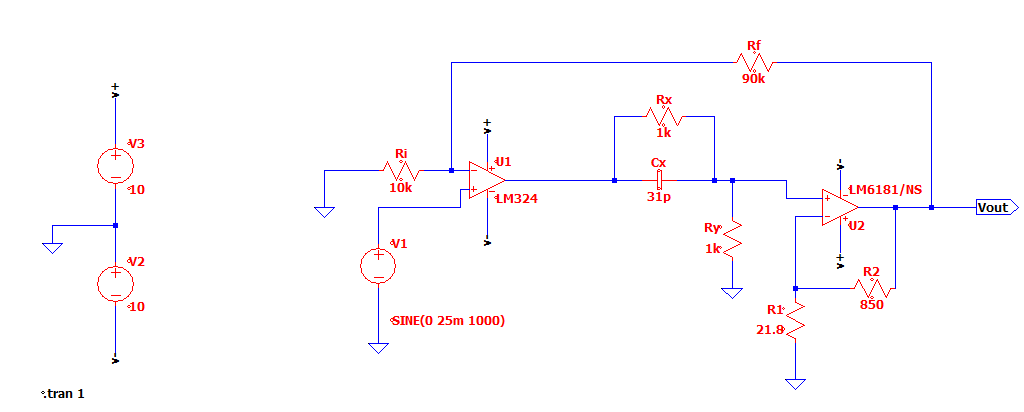
\includegraphics[width=0.7\linewidth]{VFA-CFA-Compensado.png}
    \caption{Circuito Compensado}
    \label{fig:enter-label}
\end{figure}

\hspace{1mm} En el cual, como en el caso anterior, se le inyecta una señal sinusoidal con un valor de tensión pico de \(25~mV\) con una frecuencia de \( 1~kHz \) se obtuvieron las siguientes gráficas a la entrada (color verde) y a la salida (color azul).

\begin{figure}[H]
    \centering
    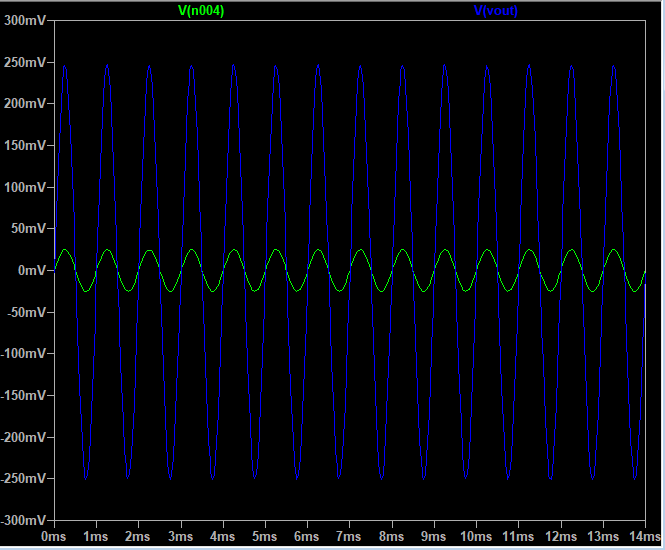
\includegraphics[width=0.7\linewidth]{VFA-CFA-Ganancia-Comp}
    \caption{Ganancia del circuito compensado.}
\end{figure}

\hspace{1mm} En donde se puede comprobar que para un valor de entrada de \( 25~mV \) se obtiene a la salida \( 250mV\). Se calcula la ganancia con los valores medidos

\begin{equation}
    G = \frac{250~mV}{25~mV}
\end{equation}

\begin{equation}
    \boxed{
    G = 10
    }
\end{equation}

\hspace{1mm} Se genera el diagrama de Bode del circuito propuestos. En este diagrama, se observa una ganancia de \(20~dB\) y una caída de \(-3~dB\), la cual se produce a una frecuencia de \(2.79~MHz\).

\begin{figure}[H]
    \centering
    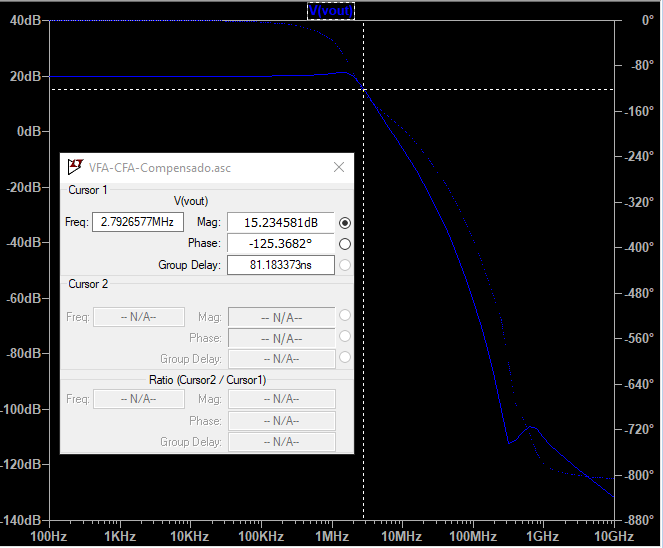
\includegraphics[width=0.7\linewidth]{VFA-CFA-Bode-Comp.png}
    \caption{Diagrama de Bode y Fase del circuito compensado}
    \label{fig:enter-label}
\end{figure}